\documentclass[
  lualatex,
  aspectratio=169,
  fleqn,
  14pt
]{beamer}

\usetheme[progressbar=frametitle]{Metropolis}
%\setbeameroption{show notes on second screen=bottom}

\usepackage{xparse}
\usepackage{mathtools,amssymb}
\usepackage{graphicx,xcolor}
\usepackage{pxrubrica}
\usepackage{calc}
\usepackage[absolute,overlay]{textpos}
%\usepackage{enumitem}
\usepackage[1.7]{bxpdfver}
\usepackage{pdfcomment}
\usepackage{ulem}
\usepackage{stackengine}
\usepackage{appendixnumberbeamer}
\usepackage{tabto}

% フォント
\usepackage[lining,tabular,sfdefault]{FiraSans}
\usepackage[mathrm=sym,mathbf=sym]{unicode-math}
\setmathfont{Fira Math}
\usepackage[no-math,deluxe,haranoaji]{luatexja-preset}
\RenewDocumentCommand\kanjifamilydefault{}{\gtdefault}

% 打ち消し線関連
\RenewDocumentCommand\ULthickness{}{.1\zh}
% 二重打ち消し
\NewDocumentCommand\dsout{m}{%
  \stackengine{.2\zh}{#1}{%
    \stackengine{-.3\zh}{\sout{\hphantom{#1}}}{\sout{\hphantom{#1}}}{O}{c}{F}{F}{L}%
  }{O}{c}{F}{F}{L}}

% 下に文字置くやつ
\NewDocumentCommand\replace{mm}{%
  \smash{\stackengine{-1\zh}{\dsout{#1}}{#2}{O}{c}{F}{F}{L}}}

% 床関数
\DeclarePairedDelimiter\floor\lfloor\rfloor

\usepackage{hyperref}

\title{%
  \texorpdfstring{%
    {\small \hspace{0.19em}ITエンジニアのための}\\[-.2\baselineskip]
    機械式計算器入門}
    {ITエンジニアのための機械式計算器入門}}
\subject{エンジニア作業飲み集会\#XXX}
\author[KusaReMKN]{上羽 未栞(a.k.a. KusaReMKN)}
\institute{%
  \url{https://KusaReMKN.com/}\\
  Twitter: \href{https://twitter.com/KusaReMKN}{@KusaReMKN}}
\keywords{機械式計算機; 機械式計算器; タイガー計算器}
\date{2025-08-08}

\begin{document}

\begin{frame}
  \titlepage
  \note{
    はじまるよ〜。

    ITエンジニアのための機械式計算器入門と題して上羽未栞が発表するよ。
  }
\end{frame}

\begin{frame}
  \frametitle{今回のおはなし}

  %~\\[-.25\baselineskip]
  \tableofcontents
  \note{
    今回の発表の流れはこんな感じだよ。
    おおよそ25分くらいで進められたらいいな。

    機械式計算器の操作を眺めながら
    現代の電子計算機に通ずる部分があることを紹介していくよ。

    四則演算に加えて平方根も計算できるので、
    百均に売っている電卓と同程度の計算能力を持っていると主張しておくよ。
    機械式計算器もナメたもんじゃないなと思ってもらえると嬉しいな。
  }
\end{frame}

\section*{みかんちゃんについて}
\note{
  まずは自己紹介するよ〜。
}

\begin{frame}
  \frametitle{自称・大天才美少女プログラミング初心者}

  \begin{textblock*}{0.5\paperwidth}(-0.3cm, 3.3cm)
    
\includegraphics[width=0.35\paperwidth]{./images/mikanchan.png}
  \end{textblock*}
  \begin{columns}
    \begin{column}{0.30\textwidth}
      \\~\\[-.25\baselineskip]
    \end{column}
    \begin{column}{0.69\textwidth}
      \\~\\[-.25\baselineskip]
      「\ruby{上羽}{うわ|ば} \ruby{未栞}{み|かん}」
      あるいは「\ruby[g]{KusaReMKN}{くされみかん}」\\
      \hspace{1.5\zw}\textbf{みかんちゃん}って呼んでね!
      \\~\\[-.5\baselineskip]

      実はプログラマでもエンジニアでもない\\
      \hspace{1.5\zw}古い計算機っぽいものが大好き\\
      \hspace{1.5\zw}自分の得意分野がわからなくなってきた
      \\~\\[-.5\baselineskip]

      Twitterで思想を垂れ流すことが得意\\
      \hspace{1.5\zw}\url{https://kusaremkn.com/}も見てね
    \end{column}
  \end{columns}
  \note{
    自称大天才美少女プログラミング初心者の上羽未栞だよ。
    みかんちゃんって呼ばれると大変喜ぶよ。

    大天才とか偉ぶっているけれど、実はプログラマでもエンジニアでもないよ。
    古い計算機っぽいものが大好きで、いろいろなものに手を出し続けていたら、
    最近は自分の得意分野が何だったのかわからなくなってきたよ。

    Twitterや自分のウェブサイトで思想を垂れ流すのが得意だよ。
    暇な人は眺めてみてね。
  }
\end{frame}

\section{機械式計算器ってなに?}
\note{
  本題に入っていくよ。
  機械式計算器についてお話するよっちゅわれても
  機械式計算器って何じゃいってなるん人もいるので、
  これについて軽く紹介していくよ。
}

\begin{frame}
  \frametitle{こんなやつ}

  \begin{textblock*}{0.5\paperwidth}(.575\paperwidth, 4\baselineskip)
    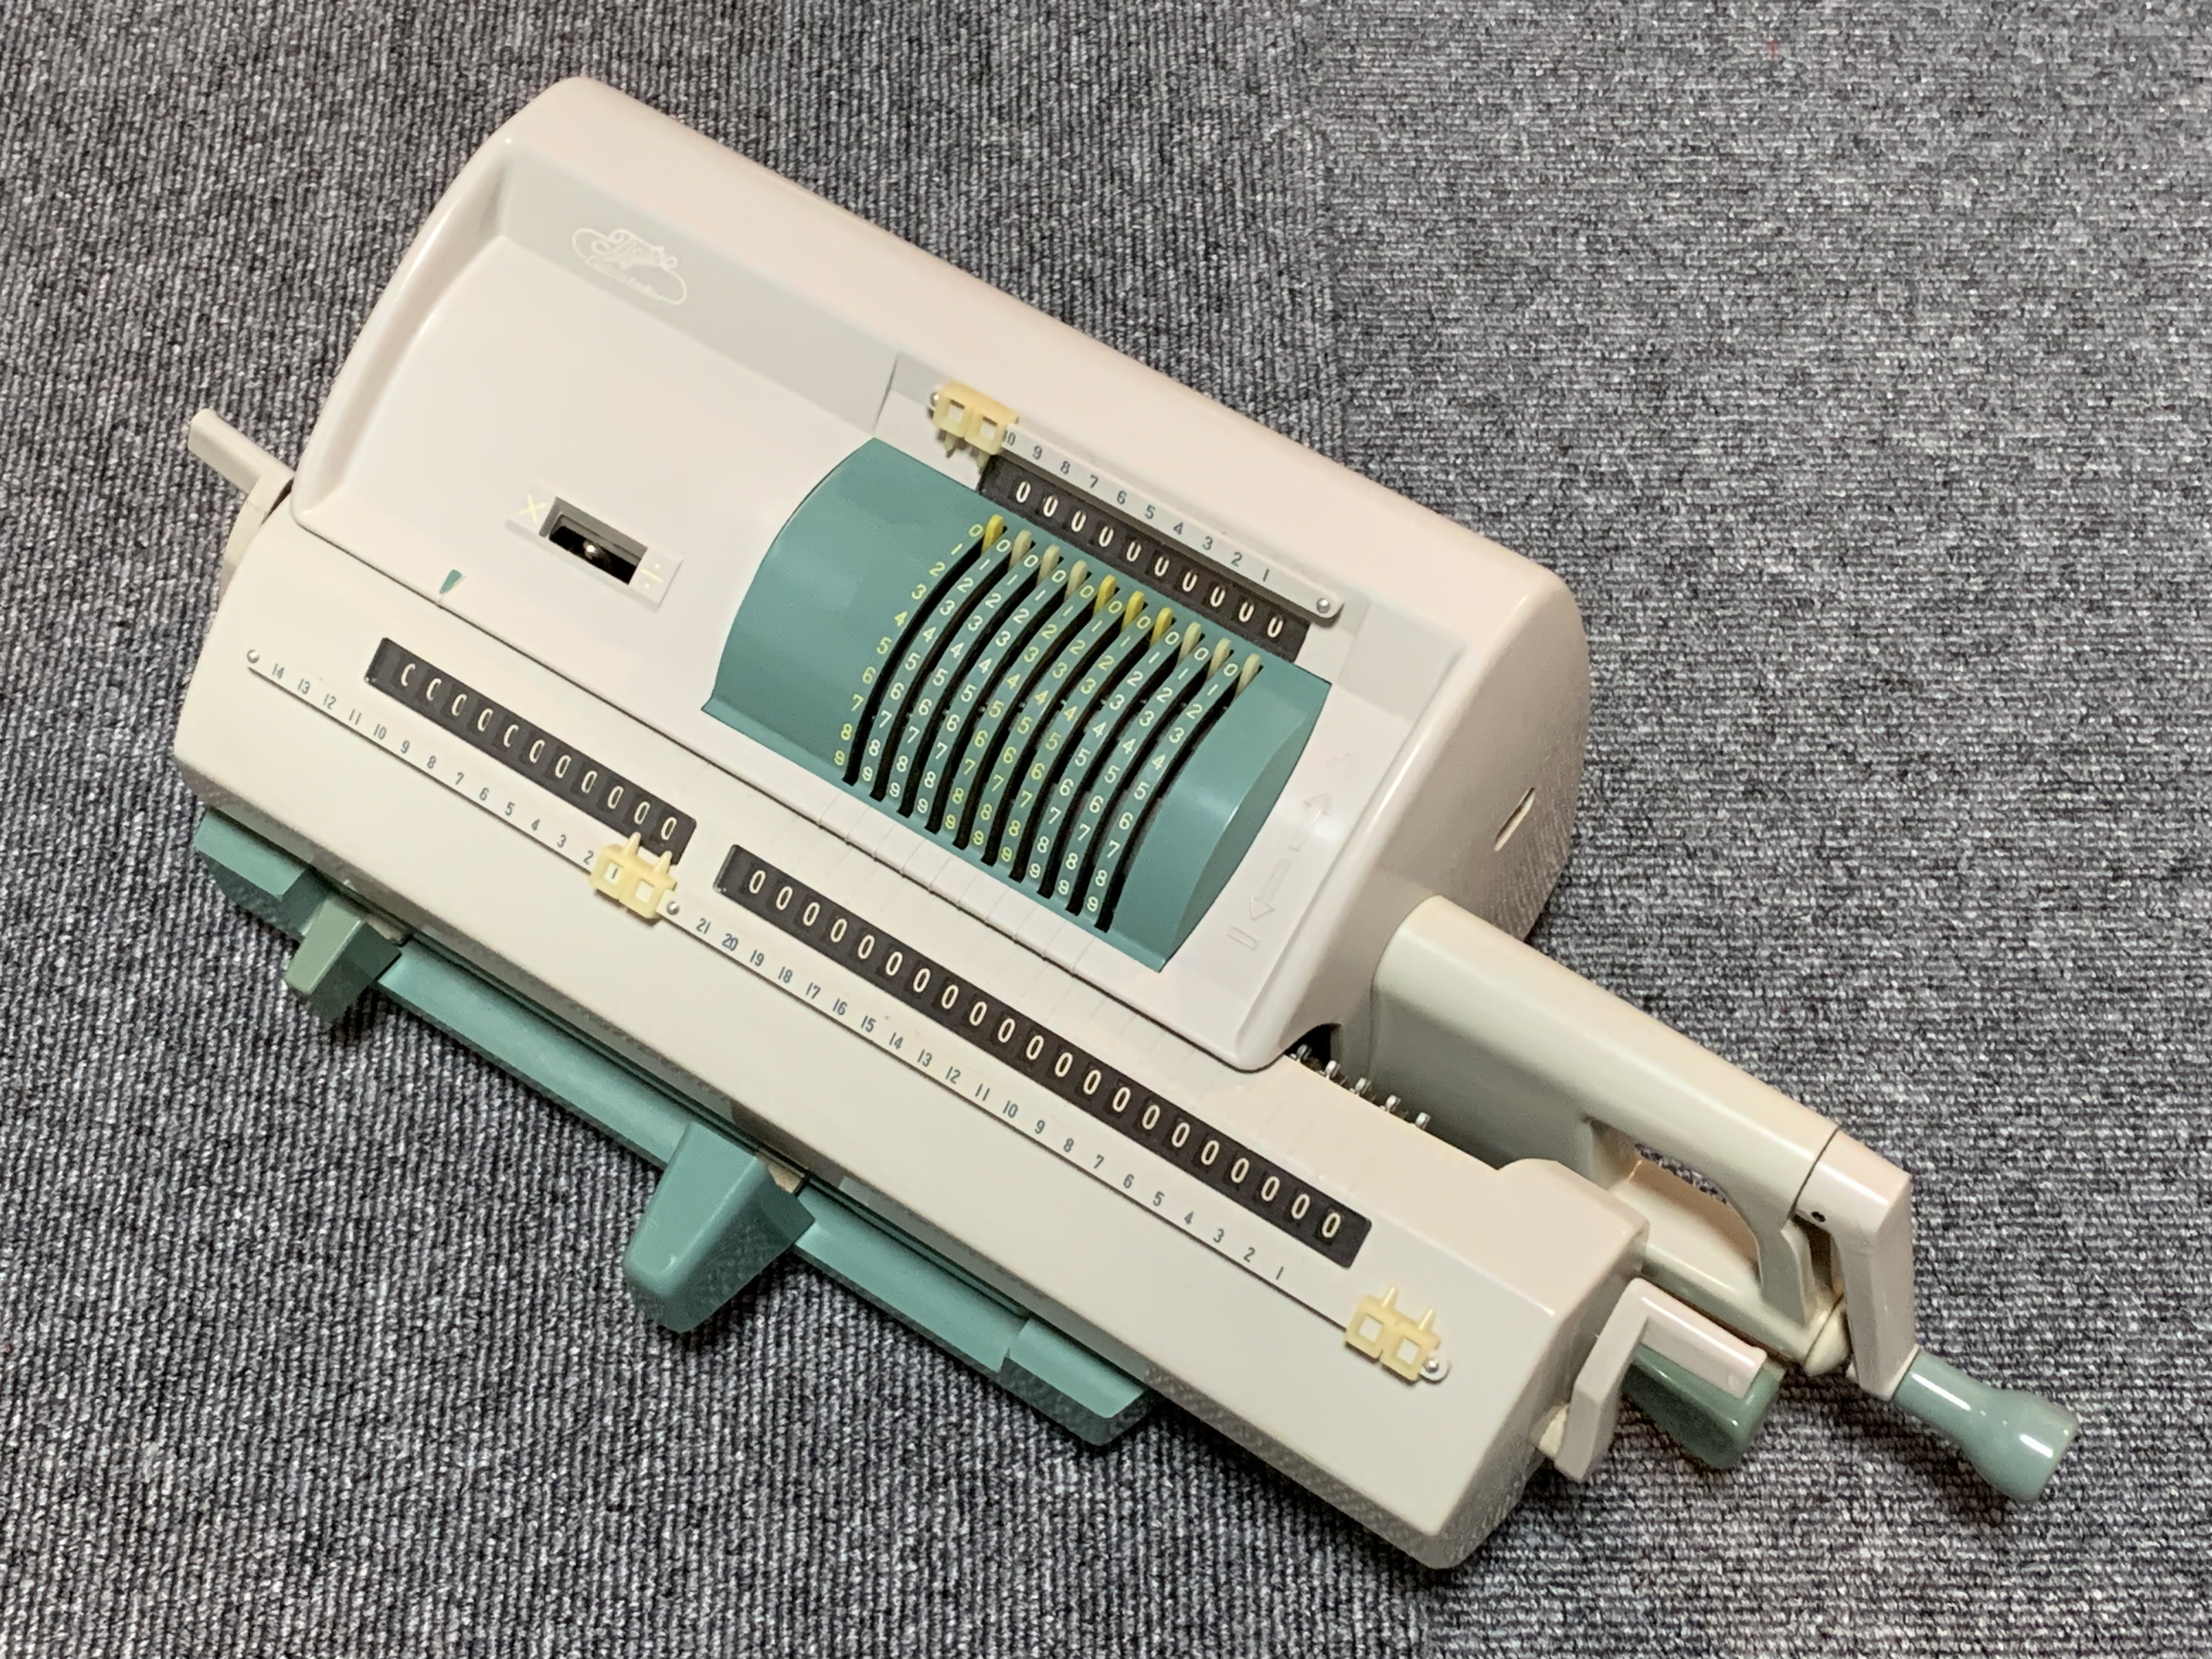
\includegraphics[width=0.375\paperwidth]{./images/IMG_6973.jpeg}
  \end{textblock*}

  電気を使わない省エネ仕様\\
  \hspace{1.5\zw}SDGsにも対応している(諸説)

  日本の会社から発売されており\\
  \hspace{1.5\zw}\textbf{タイガー計算器}として知られる

  最後の機械式計算器は1970年発売\\
  \hspace{1.5\zw}同年に電電公社がDIALSを開始\\
  \hspace{1.5\zw}まだ電卓はデカくて高かった

  \note{
    画面の右側に表示されているものが機械式計算器だよ。
    機械式計算器と銘打っているだけあって、
    ギヤやカムなどの機械的な機構を用いて計算を実現するよ。
    電気を用いない省エネ仕様であるから、今流行りのSDGsにも対応しているよ。

    この機械式計算器は、大本虎治郎っちゅう日本人が発明したものだよ。
    虎印計算器とかタイガー計算器とかって名前で発売されていたよ。

    この機械式計算器は末期のもので、1970年に発売されたものだよ。
    これは電電公社がDIALSという電話を用いた計算サービスを提供開始したのと同じ年だよ。
    Intel 4004が発売される前であることを考えると、
    当時まだ電卓というものがいかにデカくて高いものであったのか想像できると思うよ。
  }
\end{frame}

\begin{frame}
  \frametitle{計算器の外観}

  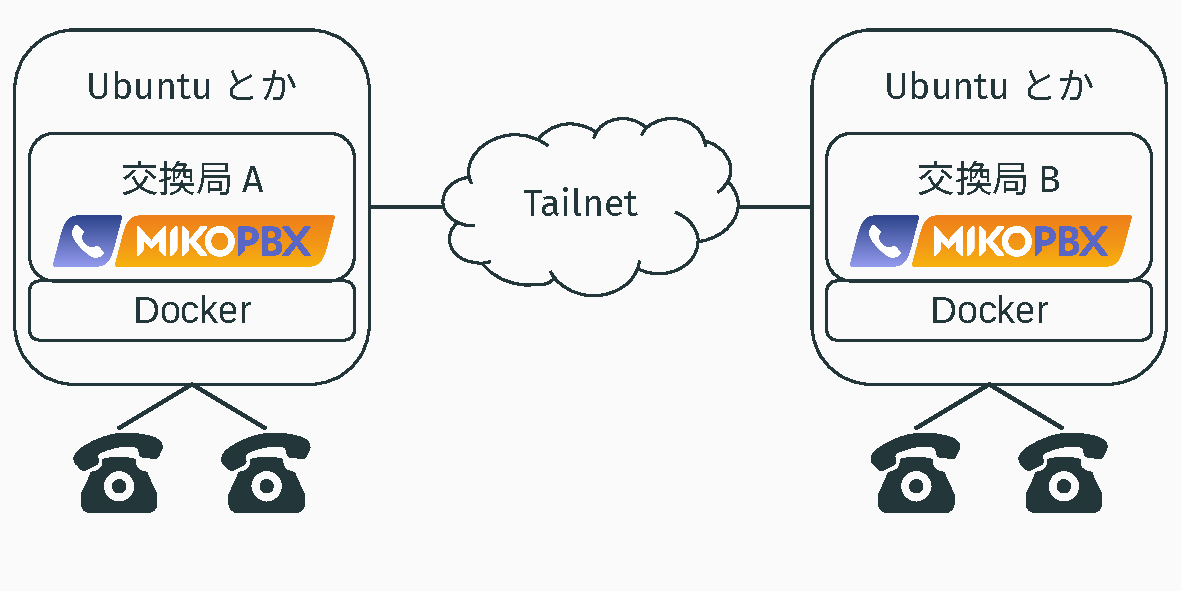
\includegraphics[page=1,width=\linewidth]{./images/pictures.pdf}

  \note{
    計算器をもう少し詳細に眺めてみるよ。
  }
\end{frame}

\begin{frame}
  \frametitle{数値の入力に関連する部分}

  \includegraphics[page=2,width=\linewidth]{./images/pictures.pdf}

  \note{
    まずは計算する数値を入力する部分だよ。
    数を入力するには「置数レバー」を操作するよ。
    見づらいかもしれないけれど、3桁毎に白色と黄色とで塗り分けられていて、
    どの桁であるのかわかりやすくなっているよ。

    入力した数は「チェックダイヤル」に表示されるよ。

    入力した数をクリアするには「レバークリア」を押し込むよ。
  }
\end{frame}

\begin{frame}
  \frametitle{演算操作に関連する部分}

  \includegraphics[page=3,width=\linewidth]{./images/pictures.pdf}

  \note{
    次は入力した数を用いて実際に演算を行う部分だよ。
    右側についている「クランクハンドル」をぐるぐる廻して計算を行うよ。
    ハンドルを前方向に廻すと加算、後ろ方向に廻すと減算を行うよ。
    また、最初にハンドルを廻した方向に応じて、「クラッチ」が自動的に設定されるよ。
    これは乗除算を行う上で重要になる部分で、ハンドルを廻した回数をカウントする方向を制御するよ。
  }
\end{frame}

\begin{frame}
  \frametitle{演算結果に関連する部分}

  \includegraphics[page=4,width=\linewidth]{./images/pictures.pdf}

  \note{
    演算結果を表示する部分についてお話するよ。
    計算結果は下側二つのダイヤルに表示されるよ。
    右側のダイヤルはハンドルを廻すと置数レバーの値が足し込まれる部分だよ。
    左側のダイヤルはハンドルを廻した回数をカウントする部分だよ。
    それぞれのダイヤルを零にするための帰零ハンドルがあるよ。
    これらのダイヤルの桁の位置をズラすことができるよ。
    これを制御するのが……
  }
\end{frame}

\begin{frame}
  \frametitle{連続乗算や桁送りに関連する部分}

  \includegraphics[page=5,width=\linewidth]{./images/pictures.pdf}

  \note{
    桁送りのレバーだよ。
    また、連続して乗算したいとき($2\times3\times4\times\cdots$みたいな)に使う
    「連乗用ツマミ」もあるよ。
  }
\end{frame}

\begin{frame}
  \frametitle{ちょっとカッコつけて呼ぶことにする}

  \includegraphics[page=6,width=\linewidth]{./images/pictures.pdf}

  \note{
    各ダイヤルについて、カッコつけて呼ぶことにするよ。
    チェックダイヤルをデータ、
    右ダイヤルをアキュムレータ、
    左ダイヤルをカウンタと呼ぶことにするよ。
  }
\end{frame}


\section{基本の操作(加減算)}
\note{
  これらを操作して簡単な加減算を実践してみるよ〜。
}

\begin{frame}
  \frametitle{簡単な足し算}

  $314+159=473$を計算するには……

  \begin{enumerate}
    \item
      全てのダイヤルをクリアする
    \item
      データに$314$を置く
    \item
      アキュムレータに足し込む($0+314$)
    \item
      データに$159$を置く
    \item
      アキュムレータに足し込む($314+159$)
    \item
      アキュムレータを読む($473$を得る)
  \end{enumerate}

  \note{
    まずは簡単な足し算を計算してみよう。
    $314+159$を計算するにはこのような手順で操作するよ。
    動画って再生できるのかな……
  }
\end{frame}

\begin{frame}
  \frametitle{簡単な引き算}

  $314-159=155$を計算するには……

  \begin{enumerate}
    \item
      全てのダイヤルをクリアする
    \item
      データに$314$を置く
    \item
      アキュムレータに足し込む($0+314$)
    \item
      データに$519$を置く
    \item
      アキュムレータから\textbf{差し引く}($314-159$)
    \item
      アキュムレータを読む($155$を得る)
  \end{enumerate}

  \note{
    続いて簡単な引き算を計算してみよう。
    $314-159$を計算するにはこのような手順で操作するよ。
    $159$を入力した後にハンドルを逆方向に廻すことがポイントだよ。
  }
\end{frame}

\begin{frame}
  \frametitle{負の数の扱い}

  $217-828=-611$を計算するには……

  \begin{enumerate}
    \item
      全てのダイヤルをクリアする
    \item
      データに$217$を置く
    \item
      アキュムレータに足し込む($0+217$)
    \item
      データに$828$を置く
    \item
      アキュムレータから\textbf{差し引く}($217-828$\hspace{1\zw}ベルが鳴る)
    \item
      アキュムレータを読む($\cdots999999389$を得る?)
  \end{enumerate}

  \note{
    結果が負になる引き算を計算してみよう。
    $217-828$を計算するにはこのような手順で操作するよ。
    $828$を入力した後にハンドルを逆方向に廻すと、
    ベルが鳴って沢山の9が表示されるよ。
    機械式計算器は結果が負になる計算を扱えないのかな?
    だから滅ぶんだよ。
  }
\end{frame}

\begin{frame}
  \frametitle{復習の時間: 負の数と2の補数}

  コンピュータは2進数の世界にある\\
  \hspace{2.5\zw}→ 負の数はしばしば\textbf{2の補数}で表現される

  $-45$について考えると……

  \begin{enumerate}
    \item
      $45$を2進数で表現する
      \tab$\cdots000101101$
    \item
      各ビットを反転する
      \tab$\cdots111010010$(1の補数)
    \item
      $1$を足す
      \tab$\cdots111010011$(2の補数)
  \end{enumerate}

  ここで手順 2. について\\
  \hspace{2.5\zw}各桁の数と$1=2-1$との差を取っていると考える

  \note{
    ここで、現代のコンピュータの負の数の扱いについて思い出してみよう。
    コンピュータは0と1との2つの数で数を表現する2進数の世界にあるよ。
    この中で負の数を表現するために、しばしば2の補数表現が用いられるよ。

    $-45$を2の補数表現で表す方法をスライドに示しているよ。
    ここで、手順の 2. について、
    これはビットを反転しているというよりも
    むしろ$1$($2-1$)との差を取っていると考えるとより一般的だよ。
  }
\end{frame}

\begin{frame}
  \frametitle{負の数と10の補数}

  機械式計算器は10進数の世界にある\\
  \hspace{2.5\zw}→ 負の数は\textbf{10の補数}で表現される

  $-611$について考えると……

  \begin{enumerate}
    \item
      $611$を10進数で表現する
      \tab$\cdots000000611$
    \item
      各桁を反転する($9$との差)
      \tab$\cdots999999388$(9の補数)
    \item
      $1$を足す
      \tab$\cdots999999389$(10の補数)
  \end{enumerate}

  $\cdots999999389$は計算器の結果に一致している\\
  \hspace{2.5\zw}→ きちんと計算できていた!

  \note{
    機械式計算器の世界に戻って来よう。
    機械式計算器は0から9までの10個の数字で数を表現する10進数の世界にあるよ。
    この中で負の数を表現するために、10の補数表現が用いられるよ。

    $-611$を10の補数表現で表す方法をスライドに示しているよ。
    2進数における2の補数表現と全く同じ手順であることがわかるよ。

    $-611$を10の補数表現で表すと$\cdots999999389$となるよ。
    これは計算器の結果に一致しているから、きちんと計算できていたことになるよ。
    なんだ、ちゃんと使えるんだね。
  }
\end{frame}

\section{ちょっと複雑な計算(乗除算)}
\note{
  加減算の方法を心得たので、次はちょっと複雑な計算にも挑戦してみよう。
}

\begin{frame}
  \frametitle{掛け算は足し算の強い版}

  $2\times3=2+2+2$\\
  \hspace{2.5\zw}→ 足し算を沢山するとよさそう

  \begin{enumerate}
    \item
      全てのダイヤルをクリアする
    \item
      データに$2$を置く
    \item
      以下を繰り返す
      \begin{enumerate}
        \item
          アキュムレータに足し込む
        \item
          カウンタを読み、
          $3$に等しかったら繰り返しをやめる
      \end{enumerate}
    \item
      アキュムレータを読む
  \end{enumerate}

  \note{
    掛け算について考えてみるよ。
    例えば、$2\times3$は$2+2+2$と書き表せるので、
    足し算を沢山行うことで実現できそうだよ。

    この手順はスライドのようになるよ。
  }
\end{frame}

\begin{frame}
  \frametitle{「掛け算は足し算の強い版」の問題点}

  $2\times3 = 2+2+2$\\
  \hspace{2.5\zw}→ 耐えられる

  $987286\times310473 = 987286+987286+987286+987286+\cdots$\\
  \hspace{2.5\zw}→ やりたくない

  \note{
    この方法は大変単純明解であるものの、
    大きな数を扱う計算では問題があるよ。
    このような計算をぐるぐると行っていたのでは、
    翌日の筋肉痛に苦しむことになりますからね。
  }
\end{frame}

\begin{frame}
  \frametitle{復習の時間: マイコンにおける掛け算の処理}

  $45\times10$について考えてみる

  ループを使って10回足し算する(簡単だけど遅い)
  \[
    45\times10 = \sum_{k=1}^{10} 45 = \underbrace{45+45+45+\dots+45}_{\text{10回}}
  \]

  シフト演算(高速な$2^n$の乗除算)を使うと計算回数を減らせる
  \[
    45\times10 = [45\times(1+2^2)]\times2^1 = [45 + (45 << 2)] << 1
  \]

  \note{
    ここで、古いコンピュータやマイコンで用いられる
    掛け算の処理について考えてみるよ。
    $45\times10$の計算を考えてみよう。

    コンピュータで計算をするなら腕を酷使することはないから、ループを廻すことは容易いよ。
    でも、この方法だとループの回数だけ計算を行うので遅くなりがちだよ。
    $45\times10$を計算すると、加算を9, 10回する必要があるよ。

    そのため、シフト演算と呼ばれる高速な$2^n$の乗除算と加算とを組み合わせることで
    高速に乗算を実装することがあるよ。
    $45\times10$を計算すると、1回の加算と2回のシフト演算によって実現できるよ。
    ここで、掛け算をしようとしているのに
    掛け算を使っているのはズルいんじゃないかと言われそうなので……
  }
\end{frame}

\begin{frame}
  \frametitle{シフト演算は文字通りシフトしているだけ}

  $45+(45<<2)$の部分を2進数で見てみる

  \begin{math}
  \begin{array}{ccccccccc@{\hspace{4\zw}}l}
       &   &   & 1 & 0 & 1 & 1 & 0 & 1 & 45    \\
    +) & 1 & 0 & 1 & 1 & 0 & 1 &   &   & 45<<2 \\
    \hline
       & 1 & 1 & 1 & 0 & 0 & 0 & 0 & 1 & 45 + (45<<2) \\
  \end{array}
  \end{math}

  2進数の世界で$n$桁左にズレると$2^n$倍になる

  \note{
    シフト演算について軽く説明をするよ。
    名の通り数を横にズラすだけの演算だよ。
    試しに$45+(45<<2)$の部分を筆算してみるとスライドのようになるよ。
    2進数の世界では$2^n$桁左にズレると$2^n$倍されることになるよ。
  }
\end{frame}

\begin{frame}
  \frametitle{機械式計算器におけるシフト演算}

  シフト演算を用いた掛け算と同様の考え方を適用する\\
  \hspace{2.5\zw}→ 計算の回数と労力とを大幅に削減できる

  桁送りのレバーでシフトできる\\
  \hspace{2.5\zw}→ 10進数の世界で$n$桁左にズレると$10^n$倍になる

  9, 8, 7については引き算を利用するとさらにすこし削減できる\\
  \hspace{2.5\zw}$9=10-1$のように考えると2回廻すだけでよい

  \note{
    機械式計算器においても、
    シフト演算を用いた掛け算と同様の考え方を適用することで
    計算の回数を労力とを大幅に削減できるよ。

    機械式計算器では、シフト演算にあたる操作を桁送りのレバーを用いて行うよ。
    機械式計算器は10進数の世界にあるので、
    $n$桁左にズラすと$10^n$倍されることになるよ。

    9, 8, 7の大きな数については、引き算を組み合わせるともうすこしラクに計算できるよ。
    例えば、$9=10-1$であるので、一つ上の桁で一回多く足し込んでおいて、
    本来の桁で一回差し引く操作をすることで同様の結果を得られるよ。
    ハンドル操作の回数を削減できるのでお得だよ。
  }
\end{frame}

\begin{frame}
  \frametitle{割り算も同様に計算できる}

  \begin{enumerate}
    \item
      全てのダイヤルをクリアする
    \item
      割られる数をデータに置き、アキュムレータに足し込む
    \item
      カウンタをクリアする
    \item
      割る数をデータ置く
    \item
      なるべく大きな桁から順に以下を繰り返す
      \begin{enumerate}
        \item
          負にならないギリギリまで引く(引き過ぎたら足して帳消し♪)
        \item
          次の桁に行く
      \end{enumerate}
    \item
      カウンタを読めば商\\
      アキュムレータを読めば余り
  \end{enumerate}

  \note{
    割り算についても同様の方法を引き算に適用することで計算できるよ。
    より大きな桁から順番に、
    負にならないギリギリまでの引き算を繰り返すと商と余りとを得られるよ。
  }
\end{frame}

\section{もっと複雑な計算(平方根)}
\note{
  もっと複雑な計算もしていくよ〜。
}

\begin{frame}
  \frametitle{平方根を求めるための考えかた}

  1から順に$n$個の奇数を足し合わせると$n^2$になるらしい
  \[
    n^2
    = \sum_{k=1}^{n} (2k-1)
    = \underbrace{1+3+5+\cdots}_{\text{$n$個}}
  \]

  ある正の数$x$の平方根を求める\\
  \hspace{2.5\zw}1から順に{\scriptsize だいたい}$\sqrt{x}$個の奇数を足し合わせると
  {\scriptsize だいたい}$x$になる
  \[
    x
    \ge \sum_{k=1}^{\floor{\sqrt{x}}} (2k-1)
    = \underbrace{1+3+5+\cdots}_{\text{$\floor{\sqrt{x}}$個}}
  \]

  \note{
    みかんちゃんは算数が苦手なのでよくわからないけれど(証明略の言い訳)、
    1\nobreak から順に$n$個の奇数を足し合わせると、その値は$n^2$になるらしいよ。

    これを逆の方向に使ってやることで、ある正の数$x$の平方根を求められるよ。
    1から順に何個かの奇数を足し合わせると、
    その値はいつかだいたい$x$になるハズだよ。
    そのときの奇数の個数がだいたい$\sqrt{x}$だよ。
    落ち着いて奇数を数えるだけで平方根を求められるので画期的だよ。
  }
\end{frame}

\begin{frame}
  \frametitle{割り算とほとんど同様の手順で計算できる(と思っている)}

  \begin{small}
    \begin{enumerate}
      \setlength{\itemsep}{0pt}
        \setlength{\parsep}{0pt}
        \setlength{\topsep}{0pt}
      \item
        全てのダイヤルをクリアする
      \item
        対象の数をデータに置き、アキュムレータのなるべく左側に足し込む
      \item
        データおよびカウンタをクリアする
      \item
        アキュムレータを小数点から二桁ごとに区切り\\
        \hspace{2.5\zw}その最も左側にあるグループの右側の桁に1を置く
        \begin{small}
          \begin{enumerate}
            \item
              負にならないギリギリまで以下を繰り返す
              \begin{enumerate}
              \item
                アキュームレータを差し引く
              \item
                データの末尾の桁に2を足す
              \end{enumerate}
              \item
                データの末尾の桁から1引く
              \item
                次の桁に行く
          \end{enumerate}
        \end{small}
      \item
        カウンタを読む
    \end{enumerate}
  \end{small}

  \note{
    これについても割り算とほぼ同様の手順で計算できると思っているよ。
    実際にはループがひとつ増えているので手順の複雑さはかなり上がっているかも。
    でも差し引く数を数えるという今回の部分は変わっていないよ。
    人間が手順を間違えなければ正しく計算できるよ。
  }
\end{frame}

\section{でも電子計算機しか持ってないし}
\note{
  ここまで聞いてくれたみんなは思っているハズだよ。
  でも家に機械式計算器ないし、電子計算機しか持っていないし、と。
}

\begin{frame}
  \frametitle{機械式計算器シミュレータ\hspace{1\zw}つくりました}

  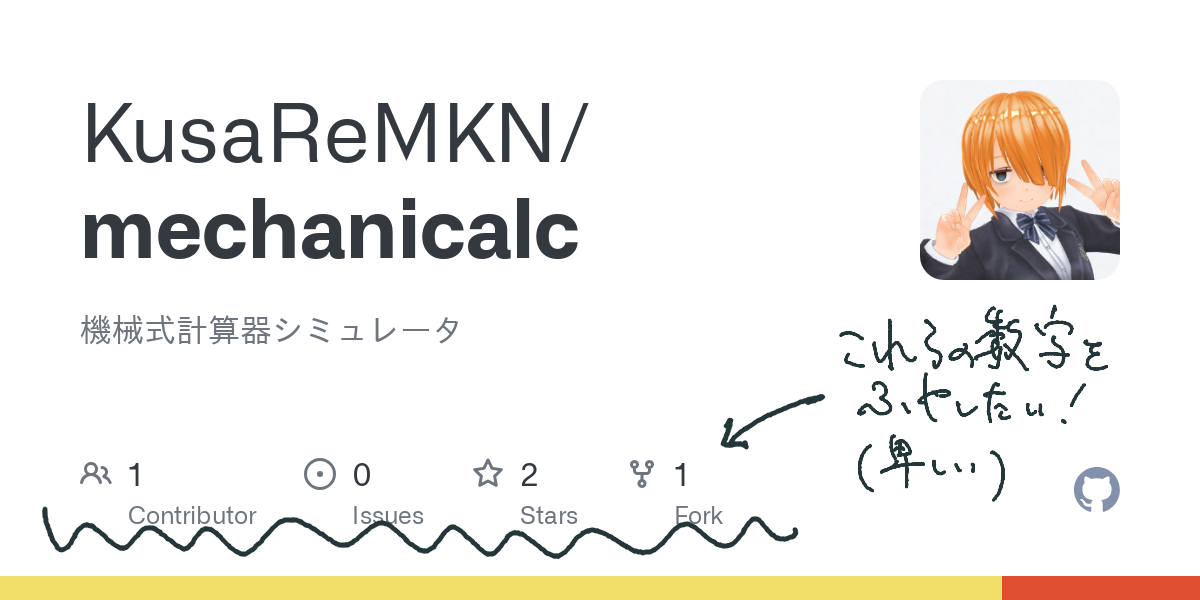
\includegraphics[width=\linewidth]{./images/mechanicalc.png}

  \note{
    そんなみんなのために機械式計算器シミュレータを作ったよ。
  }
\end{frame}

\begin{frame}
  \frametitle{Webブラウザがあれば動きます}

  \url{https://kusaremkn.github.io/mechanicalc/}

  UIが\sout{終わってる}\textbf{過度に質素}なので誰か助けて!

  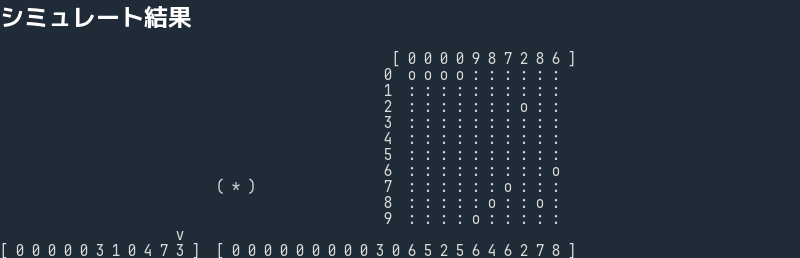
\includegraphics[width=\linewidth]{./images/simulator.png}

  \note{
    Webブラウザがあれば動作するよ。
    暇があったら試してみてね。
  }
\end{frame}

\section*{まとめ}

\begin{frame}
  \frametitle{ITエンジニアのための機械式計算器入門}

  加減算はクランクハンドルを廻すだけ\\
  \hspace{2.5\zw}負の数も補数表現を用いて扱える

  乗除算はクランクハンドルを沢山廻すだけ\\
  \hspace{2.5\zw}桁送りを活用するとラクをできる

  平方根も計算できる\\
  \hspace{2.5\zw}操作が複雑であることは否めない

  \pause
  電卓とかスマホとかでよくね?\\
  \hspace{2.5\zw}全くその通りだ!
\end{frame}

\appendix

\begin{frame}[standout]
  おわりです

  \note{
    おわりだよ〜。
  }
\end{frame}

\begin{frame}
  \frametitle{参考資料}

  \beamertemplatetextbibitems
  \begin{thebibliography}{9}
    \bibitem{1}
      株式会社タイガー.
      \newblock
      \href{https://www.tiger-inc.co.jp/temawashi/temawashi.html}
        {タイガー手廻計算器資料館}.
      \newblock{\footnotesize
      \url{https://www.tiger-inc.co.jp/temawashi/temawashi.html},\\
      (accessed 2025-08-03).\\}
    \bibitem{2}
      shiura.com.
      \newblock
      \href{https://shiura.com/unplugged/root/index.html}
        {機械式計算機による平方根の計算}.
      \newblock{\footnotesize
      \url{https://shiura.com/unplugged/root/index.html},\\
      (accessed 2025-08-03).\\}
  \end{thebibliography}
\end{frame}

\begin{frame}
  \frametitle{このスライドについて}

  Written in August 2025.

  Permanent ID of this document: \texttt{87fc40cafc05d4fe}.

  Copyright © 2025 KusaReMKN.

  特記無き場合、プログラムやソースコードは MIT License で、\\
  \hspace{1.5\zw}それ以外のコンテンツは CC-BY 4.0 で利用可能です。\\
  \hspace{1.5\zw}一部の画像には別のライセンスが適用されるかもしれません。
\end{frame}

\end{document}
% ex: se et ts=2 :
